\documentclass{beamer}
\usepackage[utf8]{inputenc}
\usepackage{graphicx, epsfig}
\usepackage{amsmath,mathrsfs,amsfonts,amssymb}
\usepackage{floatflt}
\usepackage{epic,ecltree}
\usepackage{mathtext}
\usepackage{fancybox}
\usepackage{fancyhdr}
\usepackage{multirow}
\usepackage{enumerate}
\usepackage{epstopdf}
\usepackage{multicol}
\usepackage{algorithm}
\usepackage[noend]{algorithmic}
\usepackage{tikz}
\usepackage{blindtext}
\usetheme{default}%{Singapore}%{Warsaw}%{Warsaw}%{Darmstadt}
\usecolortheme{default}

\setbeamerfont{title}{size=\Huge}
\setbeamertemplate{footline}[page number]{}

\setbeamertemplate{section in toc}[sections numbered]


\makeatletter
\newcommand\HUGE{\@setfontsize\Huge{35}{40}}
\makeatother    

\setbeamerfont{title}{size=\HUGE}
\beamertemplatenavigationsymbolsempty

% latin bold lower
\newcommand{\ba}{\mathbf{a}} 
\newcommand{\bc}{\mathbf{c}} 
\newcommand{\be}{\mathbf{e}} 
\newcommand{\bh}{\mathbf{h}} 
\newcommand{\bp}{\mathbf{p}} 
\newcommand{\bt}{\mathbf{t}} 
\newcommand{\bs}{\mathbf{s}} 
\newcommand{\bu}{\mathbf{u}} 
\newcommand{\bv}{\mathbf{v}} 
\newcommand{\bw}{\mathbf{w}} 
\newcommand{\bx}{\mathbf{x}} 
\newcommand{\by}{\mathbf{y}} 
\newcommand{\bz}{\mathbf{z}} 

% latin bold upper
\newcommand{\bA}{\mathbf{A}} 
\newcommand{\bB}{\mathbf{B}} 
\newcommand{\bC}{\mathbf{C}} 
\newcommand{\bI}{\mathbf{I}} 
\newcommand{\bL}{\mathbf{L}} 
\newcommand{\bM}{\mathbf{M}} 
\newcommand{\bQ}{\mathbf{Q}} 
\newcommand{\bT}{\mathbf{T}} 
\newcommand{\bU}{\mathbf{U}} 
\newcommand{\bV}{\mathbf{V}} 
\newcommand{\bW}{\mathbf{W}} 
\newcommand{\bX}{\mathbf{X}} 
\newcommand{\bY}{\mathbf{Y}} 
\newcommand{\bZ}{\mathbf{Z}} 

% latin cal upper
\newcommand{\cG}{\mathcal{G}} 
\newcommand{\cL}{\mathcal{L}} 
\newcommand{\cN}{\mathcal{N}} 
\newcommand{\cS}{\mathcal{S}} 
\newcommand{\cT}{\mathcal{T}} 
\newcommand{\cW}{\mathcal{W}} 
\newcommand{\cX}{\mathcal{X}} 
\newcommand{\cZ}{\mathcal{Z}} 

% latin bb upper
\newcommand{\bbE}{\mathbb{E}} 
\newcommand{\bbI}{\mathbb{I}} 
\newcommand{\bbP}{\mathbb{P}} 
\newcommand{\bbR}{\mathbb{R}} 

% greek bold lower
\newcommand{\bepsilon}{\boldsymbol{\epsilon}} 
\newcommand{\btheta}{\boldsymbol{\theta}} 
\newcommand{\blambda}{\boldsymbol{\lambda}} 
\newcommand{\bpi}{\boldsymbol{\pi}} 
\newcommand{\bmu}{\boldsymbol{\mu}} 
\newcommand{\bsigma}{\boldsymbol{\sigma}} 
\newcommand{\bphi}{\boldsymbol{\phi}} 

% greek bold upper
\newcommand{\bSigma}{\boldsymbol{\Sigma}} 

\DeclareMathOperator*{\argmin}{arg\,min}
\DeclareMathOperator*{\argmax}{arg\,max}

\newcommand{\createdgmtitle}[1]{\title[\hbox to 56mm{Deep Generative Models  \hfill\insertframenumber\,/\,\inserttotalframenumber}]
	{Deep Generative Models \\ {\Huge Lecture #1}}
	\author{Roman Isachenko}
	\institute{
\includegraphics[width=0.5cm]{../utils/ozonmasterslogo} \large{Ozon Masters}}
	\date{Spring, 2022}
}

\newcommand\myfootnote[1]{%
  \tikz[remember picture,overlay]
  \draw (current page.south west) +(1in + \oddsidemargin,0.5em)
  node[anchor=south west,inner sep=0pt]{\parbox{\textwidth}{%
      \rlap{\rule{10em}{0.4pt}}\raggedright\scriptsize \textit{#1}}};}

\newcommand\myfootnotewithlink[2]{%
  \tikz[remember picture,overlay]
  \draw (current page.south west) +(1in + \oddsidemargin,0.5em)
  node[anchor=south west,inner sep=0pt]{\parbox{\textwidth}{%
      \rlap{\rule{10em}{0.4pt}}\raggedright\scriptsize\href{#1}{\textit{#2}}}};}
      
\AtBeginSection[]
{
	\begin{frame}{Outline}
		\tableofcontents[currentsection,subsectionstyle=hide]
	\end{frame}
}
\AtBeginSubsection[]{
	\begin{frame}{Outline}
		\tableofcontents[currentsection,currentsubsection]
	\end{frame}
}
\createdgmtitle{8}
%--------------------------------------------------------------------------------
\begin{document}
%--------------------------------------------------------------------------------
\begin{frame}[noframenumbering,plain]
%\thispagestyle{empty}
\titlepage
\end{frame}
%=======
\begin{frame}{Recap of previous lecture}
	\begin{block}{Theorem}
		\vspace{-0.3cm}
		\[
			\frac{1}{n} \sum_{i=1}^n KL(q(\bz | \bx_i) || p(\bz)) = KL(q_{\text{agg}}(\bz) || p(\bz)) + \bbI_{q} [\bx, \bz],
		\]
		\vspace{-0.3cm}
	\end{block}
	
	\begin{block}{ELBO surgery}
		\vspace{-0.6cm}
		\[
		    \frac{1}{n} \sum_{i=1}^n \cL_i(q, \btheta) = \underbrace{\frac{1}{n} \sum_{i=1}^n \mathbb{E}_{q(\bz | \bx_i)} \log p(\bx_i | \bz, \btheta)}_{\text{Reconstruction loss}}
		    - \underbrace{\vphantom{ \sum_{i=1}^n} \bbI_q [\bx, \bz]}_{\text{MI}} - \underbrace{\vphantom{ \sum_{i=1}^n} KL(q_{\text{agg}}(\bz) || p(\bz))}_{\text{Marginal KL}}
		\]
	\end{block}
	\vspace{-0.8cm}
	\begin{block}{Optimal prior}
		\vspace{-0.6cm}
		\[
			KL(q_{\text{agg}}(\bz) || p(\bz)) = 0 \quad \Leftrightarrow \quad p (\bz) = q_{\text{agg}}(\bz) = \frac{1}{n} \sum_{i=1}^n q(\bz | \bx_i).
		\]
		\vspace{-0.3cm}\\
		The optimal prior distribution $p(\bz)$ is aggregated posterior $q(\bz)$.
	\end{block}
	\myfootnotewithlink{http://approximateinference.org/accepted/HoffmanJohnson2016.pdf}{Hoffman M. D., Johnson M. J. ELBO surgery: yet another way to carve up the variational evidence lower bound, 2016}
\end{frame}
%=======
\begin{frame}{Recap of previous lecture}
	\begin{block}{Optimal prior}
		\vspace{-0.6cm}
		\[
		KL(q_{\text{agg}}(\bz) || p(\bz)) = 0 \quad \Leftrightarrow \quad p (\bz) = q_{\text{agg}}(\bz) = \frac{1}{n} \sum_{i=1}^n q(\bz | \bx_i).
		\]
		\vspace{-0.4cm}\\
		The optimal prior distribution $p(\bz)$ is aggregated posterior $q(\bz)$.
	\end{block}

	\begin{block}{VampPrior}
		\vspace{-0.4cm}
		\[
		p(\bz | \blambda) = \frac{1}{K} \sum_{k=1}^K q(\bz | \bu_k),
		\]
		\vspace{-0.2cm} \\
		where $\blambda = \{\bu_1, \dots, \bu_K\}$ are trainable pseudo-inputs.
	\end{block}
	\begin{block}{Flow-based VAE prior}
		\vspace{-0.5cm}
		\[
			\log p(\bz | \blambda) = \log p(\bepsilon) + \log \det \left | \frac{d \bepsilon}{d\bz}\right| = \log p(\bepsilon) + \log \det \left | \frac{\partial f(\bz, \blambda)}{\partial \bz}\right| 
		\]
	\end{block}
	\myfootnote{\href{https://arxiv.org/abs/1705.07120}{Tomczak J. M., Welling M. VAE with a VampPrior, 2017} \\
	\href{https://arxiv.org/abs/1611.02731}{Chen X. et al. Variational Lossy Autoencoder, 2016}}
\end{frame}
%=======
\begin{frame}{Recap of previous lecture}
	\begin{block}{Standart ELBO}
		\vspace{-0.3cm}
		\[
			p(\bx | \btheta) \geq \mathcal{L} (\bphi, \btheta)  = \mathbb{E}_{q(\bz | \bx, \bphi)} \log \frac{p(\bx, \bz | \btheta)}{q(\bz| \bx, \bphi)} \rightarrow \max_{\bphi, \btheta}.
		\]
		\vspace{-0.5cm}
	\end{block}
	\begin{block}{Expressive flow-based VAE posterior}
		\vspace{-0.3cm}
		\[
			\log q(\bz^* | \bx, \bphi, \blambda) = \log q(\bz | \bx, \bphi) + \log \det \left | \frac{\partial f(\bz, \blambda)}{\partial \bz}\right|
		\]
		\vspace{-0.3cm}
	\end{block}
	\begin{block}{ELBO with flow-based posterior}
		\vspace{-0.8cm}
		\begin{multline*}
				\mathcal{L} (\bphi, \btheta, \blambda)  
				= \mathbb{E}_{q(\bz^* | \bx, \bphi, \blambda)} \bigl[\log p(\bx, \bz^* | \btheta) - \log q(\bz^*| \bx, \bphi, \blambda) \bigr] = \\
				= \mathbb{E}_{q(\bz | \bx, \bphi)} \bigg[\log p(\bx, \bz^* | \btheta) -  \log q(\bz | \bx, \bphi ) + \log \left| \det \left( \frac{\partial f(\bz, \blambda)}{\partial \bz} \right) \right| \bigg].
		\end{multline*}
		\vspace{-0.6cm}
	\end{block}
	\begin{itemize}
		\item Obtain samples $\bz$ from the encoder $q(\bz | \bx, \bphi)$.
		\item Apply flow model $\bz^* = f(\bz, \blambda)$.
		\item Compute likelihood for $\bz^*$ using the decoder, base distribution for $\bz^*$ and the Jacobian.
	\end{itemize}
	\myfootnotewithlink{https://arxiv.org/abs/1505.05770}{Rezende D. J., Mohamed S. Variational Inference with Normalizing Flows, 2015} 
\end{frame}
%=======
\begin{frame}{Recap of previous lecture}
	\begin{block}{Expressive flow-based VAE posterior}
		\vspace{-0.3cm}
		\[
			\log q(\bz^* | \bx, \bphi, \blambda) = \log q(\bz | \bx, \bphi) + \log \det \left | \frac{\partial f(\bz, \blambda)}{\partial \bz}\right|
		\]
		\vspace{-0.5cm}
	\end{block}
	\begin{block}{Expressive flow-based VAE prior}
		\vspace{-0.5cm}
		\[
			\log p(\bz | \blambda) = \log p(\bepsilon) + \log \det \left | \frac{d \bepsilon}{d\bz}\right|; \quad 
			\bz = g(\bepsilon, \blambda) = f^{-1}(\bepsilon, \blambda)
		\]
	\end{block}
	\vspace{-0.6cm}
	\begin{block}{Theorem}
	VAE with the flow-based prior for latent code $\bz$ is equivalent to VAE with flow-based posterior for latent code $\bz$.
	\end{block}
	\vspace{-0.6cm}
	\begin{align*}
		\mathcal{L}(\bphi, \btheta, \blambda) &= \mathbb{E}_{q(\bz | \bx, \bphi)} \log p(\bx | \bz, \btheta) - \underbrace{KL( q(\bz | \bx, \bphi) || p(\bz | \blambda))}_{\text{flow-based prior}} \\
		& = \mathbb{E}_{q(\bz | \bx, \bphi)} \log p(\bx | \bz, \btheta) - \underbrace{KL( q(\bz | \bx, \bphi, \blambda) || p(\bz))}_{\text{flow-based posterior}}
	\end{align*}
	\myfootnotewithlink{https://arxiv.org/abs/1611.02731}{Chen X. et al. Variational Lossy Autoencoder, 2016}
\end{frame}
%=======
\begin{frame}{Outline}
	\tableofcontents
\end{frame}
\AtBeginSection[ ]
{
	\begin{frame}{Outline}
		\tableofcontents[currentsection]
	\end{frame}
}
%=======
\begin{frame}{Dequantization}
	\begin{itemize}
		\item Images are discrete data, pixels lie in the \{0, 255\} integer domain (the model is $P(\bx | \btheta) = \text{Categorical}(\bpi(\btheta))$).
		\item Flow is a continuous model (it works with continuous data $\bx$).
	\end{itemize}
	By fitting a continuous density model to discrete data, one can produce a degenerate solution with all probability mass on discrete values. \\
	How to convert a discrete data distribution to a continuous one?
	
	\begin{minipage}[t]{0.5\columnwidth}
		\begin{block}{Uniform dequantization}
		\vspace{-0.5cm}
			\begin{align*}
				\bx &\sim \text{Categorical}(\bpi) \\
				 \bu &\sim U[0, 1]
			\end{align*}
			\[
			\by = \bx + \bu \sim \text{Continuous} 
			\]
		\end{block}
	\end{minipage}%
	\begin{minipage}[t]{0.5\columnwidth}
		\begin{figure}
			\centering
			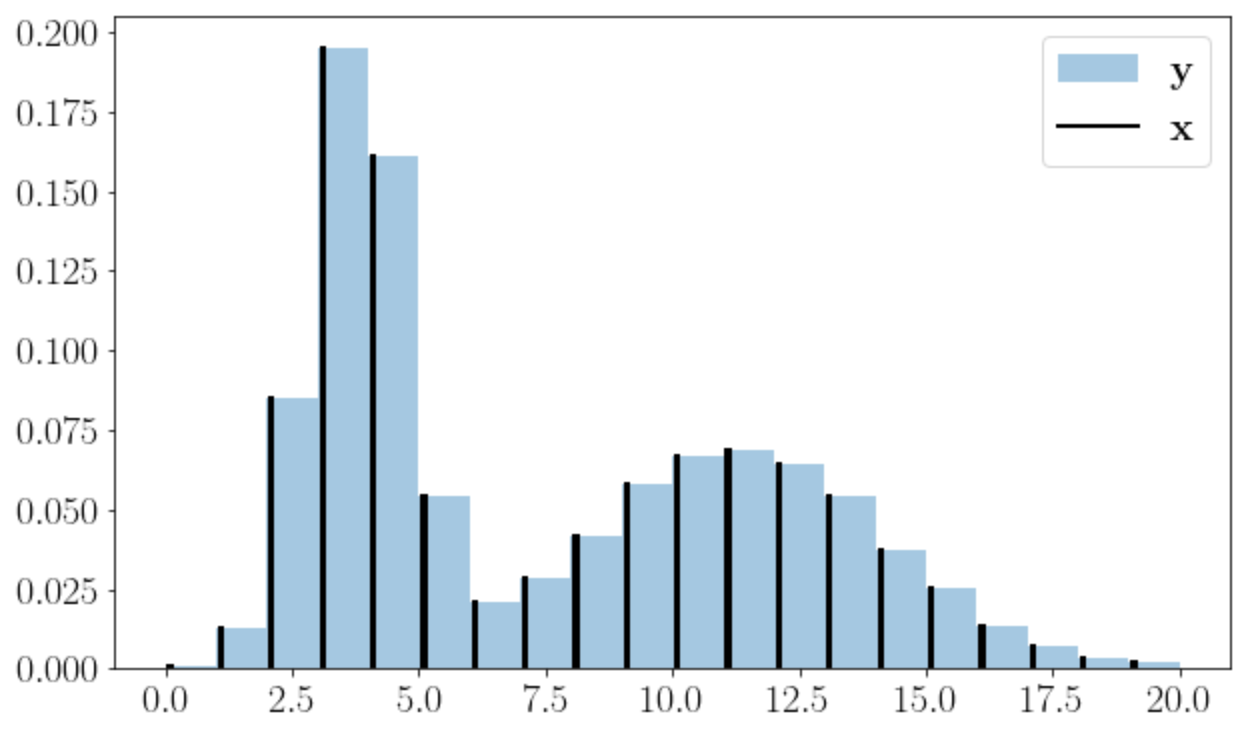
\includegraphics[width=1.0\linewidth]{figs/uniform_dequantization.png}
		\end{figure}
	\end{minipage}
	\myfootnotewithlink{https://arxiv.org/abs/1511.01844}{Theis L., Oord A., Bethge M. A note on the evaluation of generative models. 2015}
\end{frame}
%=======
\begin{frame}{Uniform dequantization}
	\begin{block}{Statement}
		Fitting continuous model $p(\by | \btheta)$ on uniformly dequantized data $\by = \bx + \bu, \, \bu \sim U[0, 1]$ is equivalent to maximization of a lower bound on log-likelihood for a discrete model:
		\vspace{-0.2cm}
		\[
		P(\bx | \btheta) = \int_{U[0, 1]} p(\bx + \bu | \btheta) d \bu
		\]
		\vspace{-0.5cm} 
	\end{block}
	\begin{block}{Proof}
		\vspace{-0.8cm}
		\begin{multline*}
			\bbE_{\pi} \log p(\by | \btheta) = \int \pi(\by) \log p(\by | \btheta) d \by = \\ 
			= \sum \pi(\bx) \int_{U[0,1]} \log p(\bx + \bu | \btheta) d \bu \leq \\
			 \leq \sum \pi(\bx) \log \int_{U[0,1]}  p(\bx + \bu | \btheta) d \bu = \\
			 = \sum \pi(\bx) \log P(\bx | \btheta) = \bbE_{\pi} \log P(\bx | \btheta).
		\end{multline*}
	\end{block}
	\myfootnotewithlink{https://arxiv.org/abs/1511.01844}{Theis L., Oord A., Bethge M. A note on the evaluation of generative models. 2015}
\end{frame}
%=======
\begin{frame}{Variational dequantization}
	\begin{minipage}[t]{0.5\columnwidth}
			\begin{figure}
				\centering
				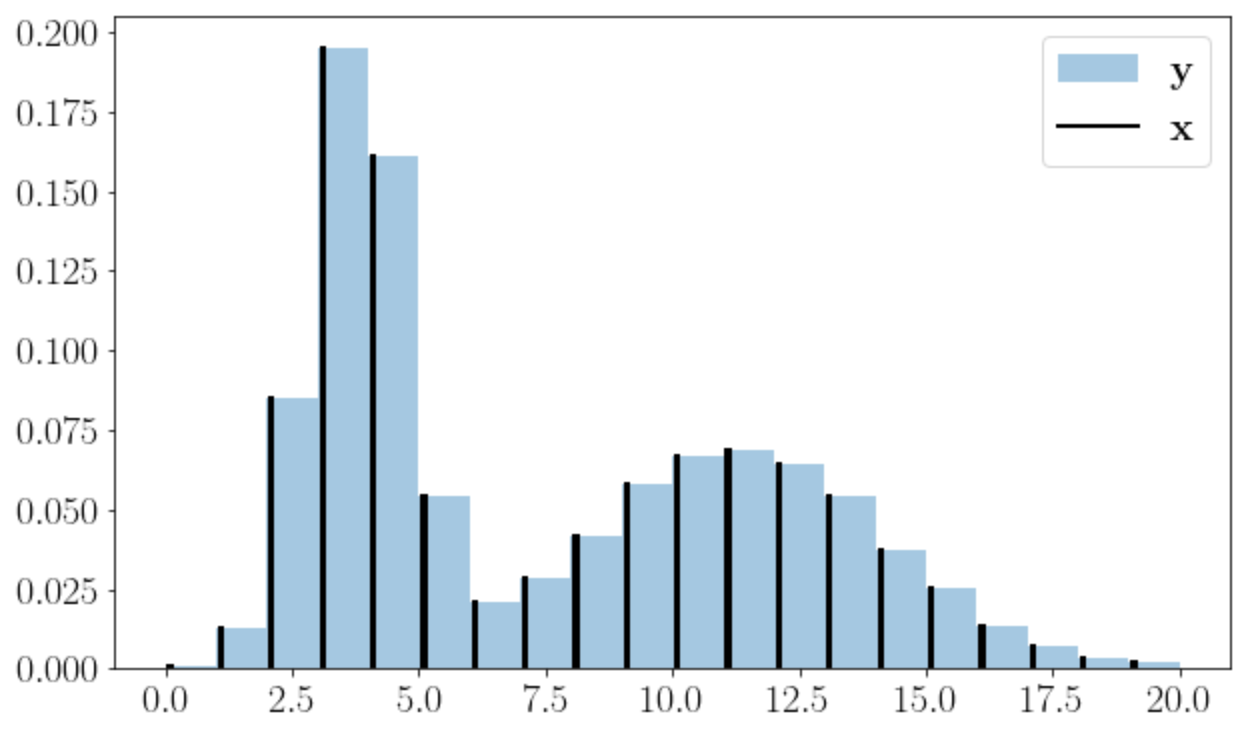
\includegraphics[width=1.0\linewidth]{figs/uniform_dequantization.png}
			\end{figure}
	\end{minipage}%
	\begin{minipage}[t]{0.5\columnwidth}
		\begin{figure}
			\centering
			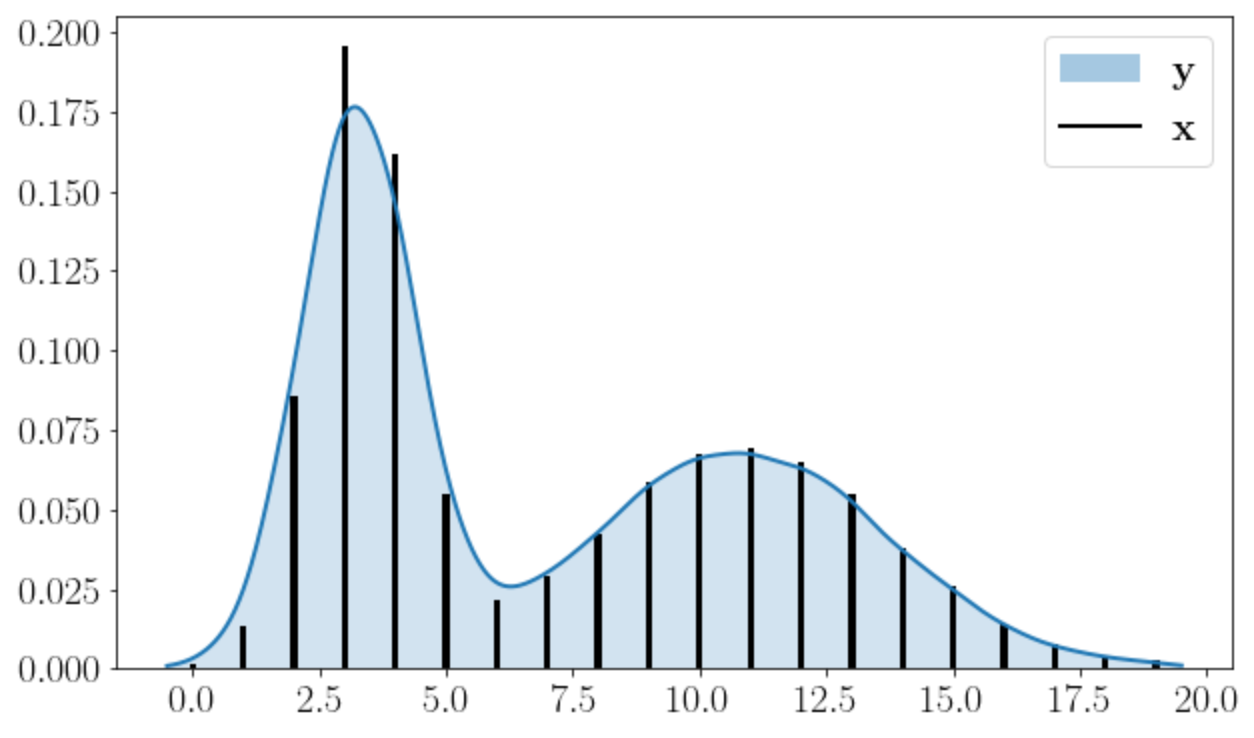
\includegraphics[width=1.0\linewidth]{figs/variational_dequantization.png}
		\end{figure}
	\end{minipage}
	\begin{itemize}
		\item $p(\by | \btheta)$ assign unifrom density to unit hypercubes $\bx + U[0, 1]$ (left fig).
		\item Neural network density models are smooth function approximators (right fig).
		\item Smooth dequantization is more natural.
	\end{itemize}
	How to perform the smooth dequantization? \\
\end{frame}
%=======
\begin{frame}{Flow++}
	\vspace{-0.3cm}
	\begin{block}{Variational dequantization}
		Introduce variational dequantization noise distribution $q(\bu | \bx)$ and treat it as an approximate posterior. 
	\end{block}
	\vspace{-0.3cm}
	\begin{block}{Variational lower bound}
		\vspace{-0.7cm}
		\begin{multline*}
		 \log P(\bx | \btheta) = \left[ \log \int q(\bu | \bx) \frac{p(\bx + \bu | \btheta)}{q(\bu | \bx)} d \bu \right] \geq \\ 
			\geq  \int q(\bu | \bx) \log \frac{p(\bx + \bu | \btheta)}{q(\bu | \bx)} d \bu = \mathcal{L}(q, \btheta).
		\end{multline*}
	\end{block}
	\vspace{-0.6cm}
	\begin{block}{Uniform dequantization bound}
		\vspace{-0.6cm}
		\[
		 \log P(\bx | \btheta) = \log \int_{U[0, 1]} p(\bx + \bu | \btheta) d \bu \geq \int_{U[0, 1]} \log p(\bx + \bu | \btheta) d \bu.
		\]
		\vspace{-0.4cm}
	\end{block}
	Uniform dequantization is a special case of variational dequantization ($q(\bu | \bx) = U[0, 1]$).
	\myfootnotewithlink{https://arxiv.org/abs/1902.00275}{Ho J. et al. Flow++: Improving Flow-Based Generative Models with Variational Dequantization and Architecture Design, 2019}
\end{frame}
%=======
\begin{frame}{Flow++}
	\vspace{-0.3cm}
	\begin{block}{Variational lower bound}
		\vspace{-0.3cm}
		\[
			\mathcal{L}(q, \btheta) = \int q(\bu | \bx) \log \frac{p(\bx + \bu | \btheta)}{q(\bu | \bx)} d \bu.
		\]
		\vspace{-0.3cm}
	\end{block}
	Let $\bu = h(\bepsilon, \bphi)$ is a flow model with base distribution $\bepsilon \sim p(\bepsilon) = \mathcal{N}(0, \mathbf{I})$:
	\vspace{-0.3cm}
	\[
		q(\bu | \bx) = p(h^{-1}(\bu, \bphi)) \cdot \left| \det \frac{\partial h^{-1}(\bu, \bphi)}{\partial \bu}\right|.
	\]
	\vspace{-0.7cm}
	\begin{block}{Flow-based variational dequantization}
		\vspace{-0.8cm}
		\[
			\log P(\bx | \btheta) \geq \cL(\bphi, \btheta) = \int p(\bepsilon) \log \left( \frac{p(\bx + h(\bepsilon, \bphi) | \btheta)}{p(\bepsilon) \cdot \left| \det \frac{\partial h(\bepsilon, \bphi)}{\partial \bepsilon}\right|^{-1}} \right) d\bepsilon.
		\]
		\vspace{-0.3cm}
	\end{block}
	If $p(\bx + \bu | \btheta)$ is also a flow model, it is straightforward to calculate stochastic gradient of this ELBO.
	\myfootnotewithlink{https://arxiv.org/abs/1902.00275}{Ho J. et al. Flow++: Improving Flow-Based Generative Models with Variational Dequantization and Architecture Design, 2019}
\end{frame}
%=======
\begin{frame}{Flow++}
	\begin{block}{Flow-based variational dequantization}
	\vspace{-0.3cm}
	\[
		\log P(\bx | \btheta) \geq \int p(\bepsilon)\log \left( \frac{p(\bx + h(\bepsilon, \bphi))}{p(\bepsilon) \cdot \left| \det \frac{\partial h(\bepsilon, \bphi)}{\partial \bepsilon}\right|^{-1}} \right) d\bepsilon.
	\]
	\end{block}
	\begin{figure}
		\centering
		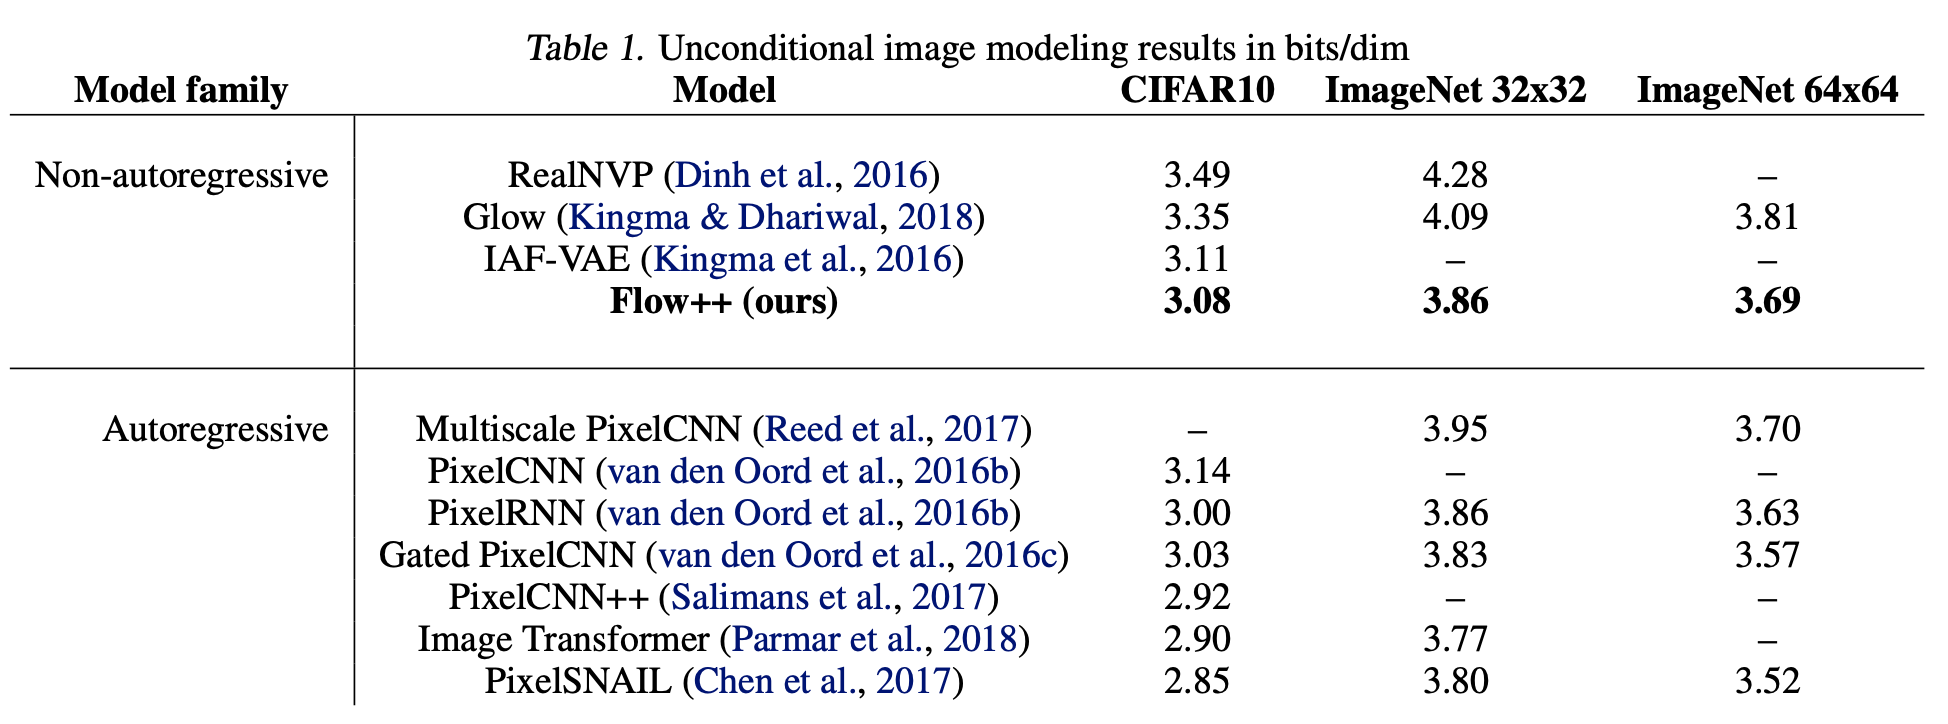
\includegraphics[width=\linewidth]{figs/flow++1.png}
	\end{figure}
	\vspace{-0.1cm}
	\myfootnotewithlink{https://arxiv.org/abs/1902.00275}{Ho J. et al. Flow++: Improving Flow-Based Generative Models with Variational Dequantization and Architecture Design, 2019}
\end{frame}
%=======
\begin{frame}{Disentangled representations}
	\textbf{Representation learning} is looking for an interpretable representation of the independent data generative factors. 
	\begin{block}{Disentanglement informal definition}
		Every single latent unit are sensitive to changes in a single generative factor, while being invariant to changes in other factors. 
	\end{block}
	\begin{block}{Generative process}
		\vspace{-0.2cm}
		\begin{itemize}
		    \item $\pi(\bx | \bv, \bw) = \text{Sim}(\bv, \bw)$~-- true world simulator;
		    \item $\bv$~-- conditionally independent factors: $\pi(\bv | \bx) = \prod_{j=1}^d \pi(v_j | \bx)$;
		    \item $\bw$~-- conditionally dependent factors. 
		\end{itemize}
	\end{block}
	\vspace{-0.3cm}
	\begin{block}{Unsupervised generative model}
		\vspace{-0.4cm}
		\[
		    p(\bx | \bz, \btheta) \approx \pi(\bx | \bv, \bw).
		\]
		The latent factors $q(\bz|\bx)$ capture the factors $\bv$ in a disentangled manner. The conditionally dependent factors $\bw$ remains entangled in a subset of $\bz$ that is not used for representing $\bv$. 
	\end{block}
	\myfootnotewithlink{https://openreview.net/references/pdf?id=Sy2fzU9gl}{Higgins I. et al. beta-VAE: Learning Basic Visual Concepts with a Constrained Variational Framework, 2017}
\end{frame}
%=======
\begin{frame}{$\beta$-VAE}
	\begin{block}{ELBO objective}
	\vspace{-0.2cm}
	\[
	    \mathcal{L}(q, \btheta, \beta) = \mathbb{E}_{q(\bz | \bx)} \log p(\bx | \bz, \btheta) - \beta \cdot KL (q(\bz | \bx) || p(\bz)).
	\]
	\vspace{-0.5cm}
	\end{block}
	What do we get at $\beta = 1$? \\
	\begin{block}{Constrained optimization}
		\vspace{-0.5cm}
		\[
			\max_{q, \btheta} \mathbb{E}_{q(\bz | \bx)} \log p(\bx | \bz, \btheta), \quad \text{subject to } KL (q(\bz | \bx) || p(\bz)) < \epsilon.
		\]
		\vspace{-0.5cm}
	\end{block}
	\begin{block}{Hypothesis}
	We are able to learn disentangled representations of the independent factors $\bv$ by setting a stronger constraint with $\beta > 1$.
	\end{block}
	\textbf{Note:} It leads to poorer reconstructions and a loss of high frequency details. 
	\myfootnotewithlink{https://openreview.net/references/pdf?id=Sy2fzU9gl}{Higgins I. et al. beta-VAE: Learning Basic Visual Concepts with a Constrained Variational Framework, 2017}
\end{frame}
%=======
\begin{frame}{$\beta$-VAE}
	\begin{figure}
	    \centering
	    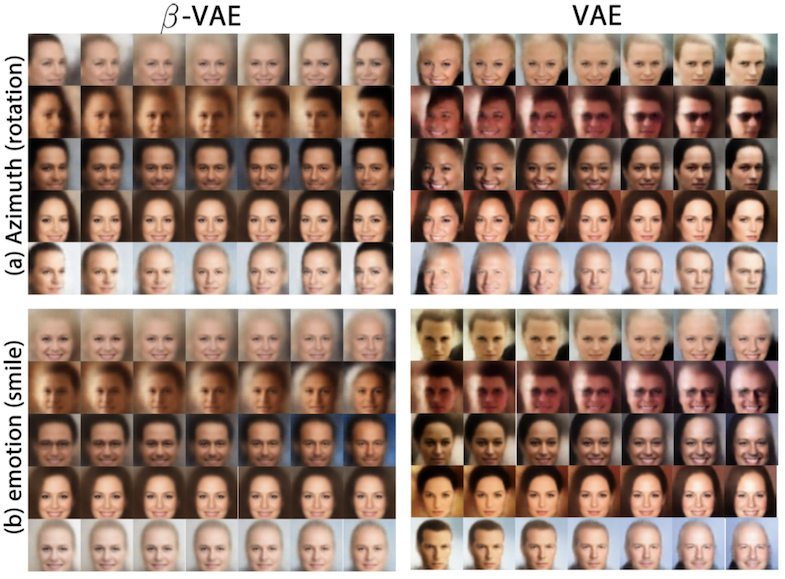
\includegraphics[width=0.9\linewidth]{figs/betaVAE_1.png}
	\end{figure}

	\myfootnotewithlink{https://openreview.net/references/pdf?id=Sy2fzU9gl}{Higgins I. et al. beta-VAE: Learning Basic Visual Concepts with a Constrained Variational Framework, 2017}
\end{frame}
%=======
\begin{frame}{$\beta$-VAE}
		\begin{figure}[h]
			\centering
			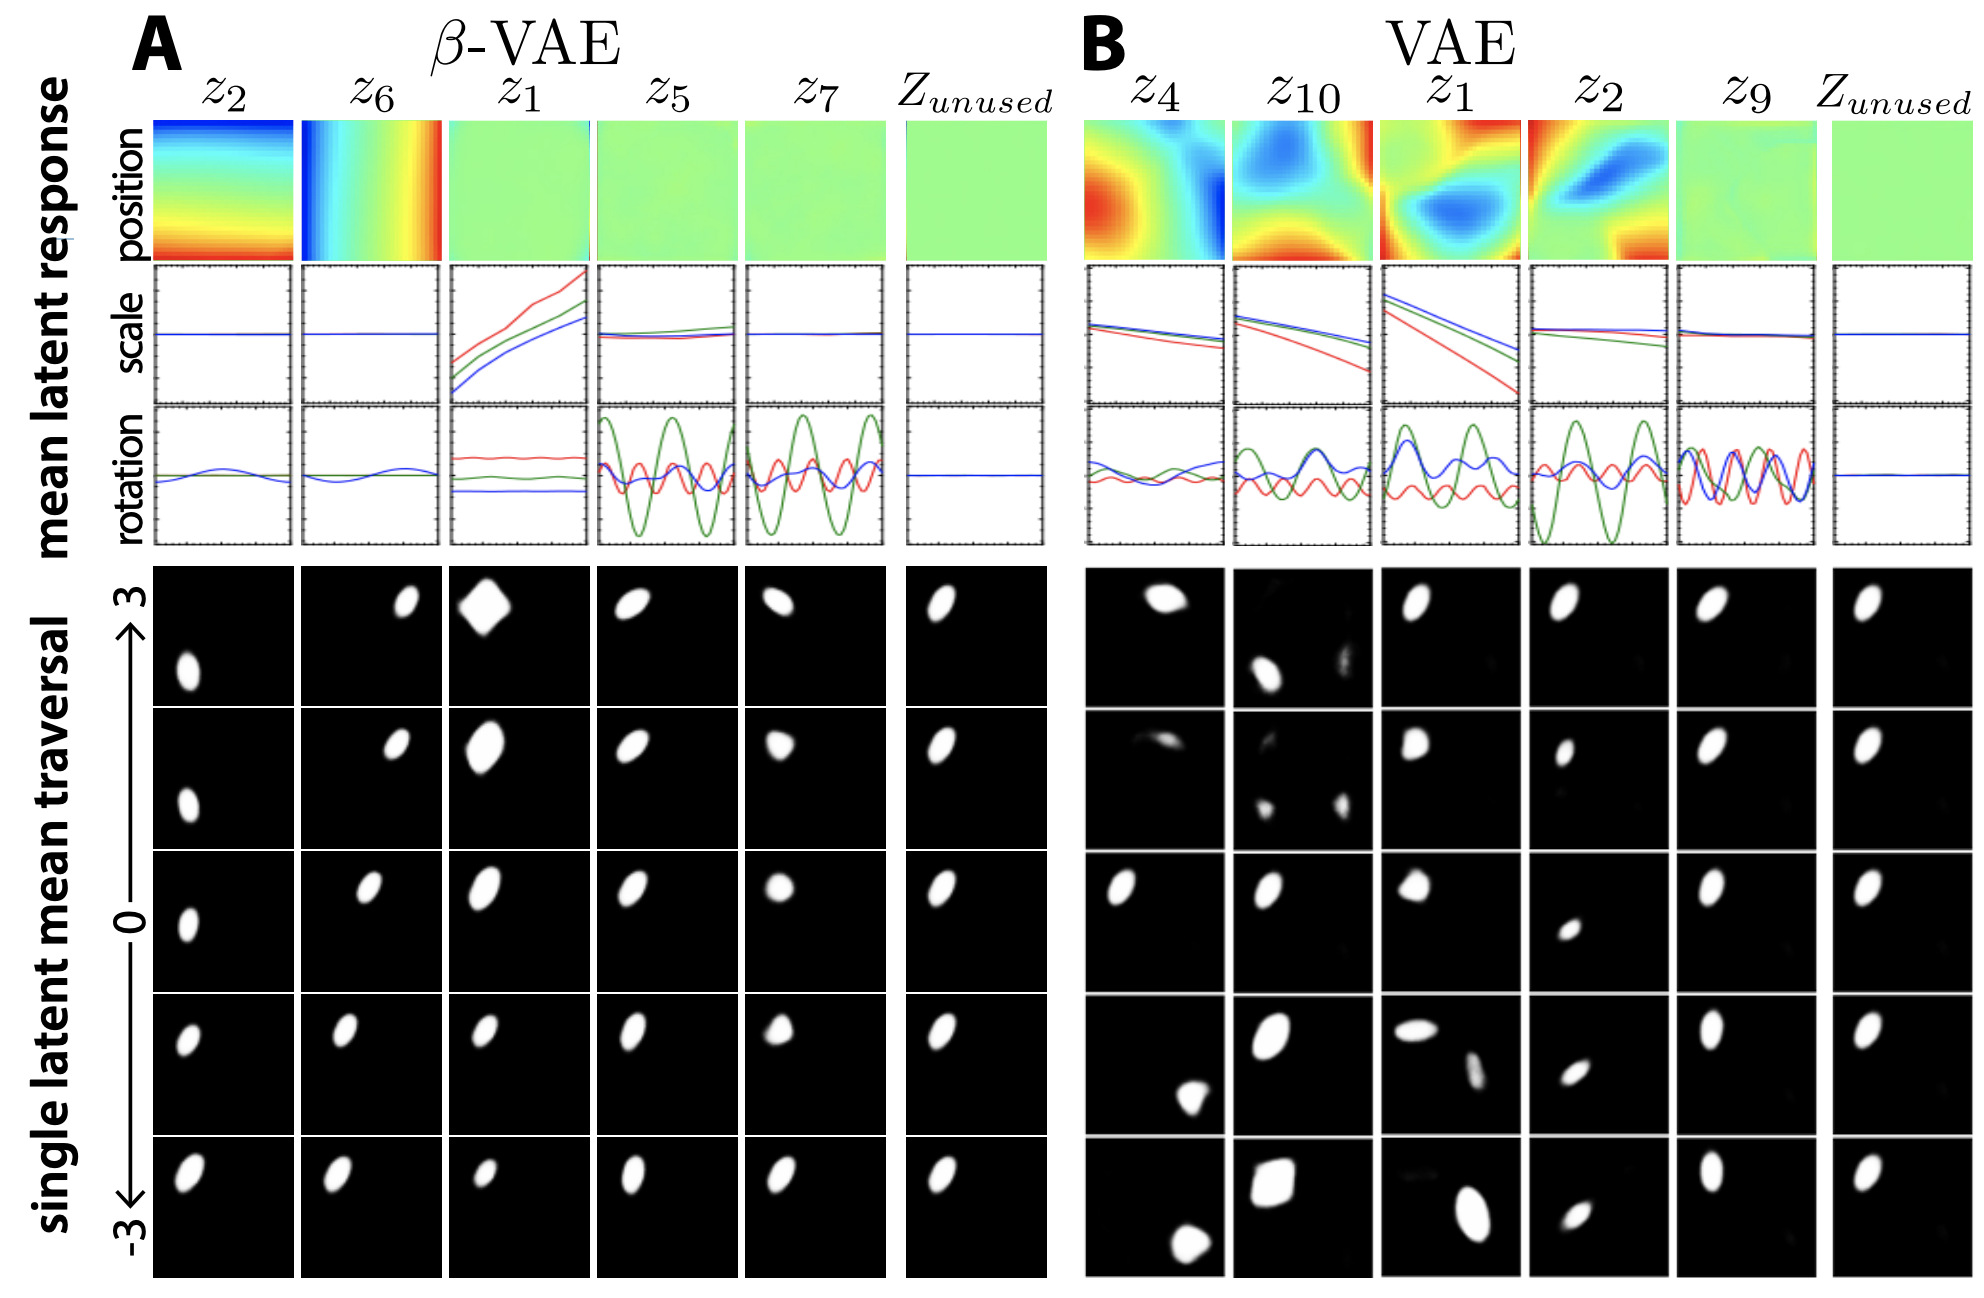
\includegraphics[width=.95\linewidth]{figs/betaVAE_5.png}
		\end{figure}

	\myfootnotewithlink{https://openreview.net/references/pdf?id=Sy2fzU9gl}{Higgins I. et al. beta-VAE: Learning Basic Visual Concepts with a Constrained Variational Framework, 2017}
\end{frame}
%=======
\begin{frame}{$\beta$-VAE}
	\begin{block}{ELBO}
		\vspace{-0.2cm}
		\[
		\mathcal{L}(q, \btheta, \beta) = \mathbb{E}_{q(\bz | \bx)} \log p(\bx | \bz, \btheta) - \beta \cdot KL(q(\bz | \bx) || p(\bz)).
		\]
		\vspace{-0.4cm}
	\end{block}
	\begin{block}{ELBO surgery}
		\vspace{-0.3cm}
		{\footnotesize
			\[
			\frac{1}{n} \sum_{i=1}^n \cL_i(q, \btheta, \beta) = \underbrace{\frac{1}{n} \sum_{i=1}^n \mathbb{E}_{q(\bz | \bx_i)} \log p(\bx_i | \bz, \btheta)}_{\text{Reconstruction loss}} - \beta \cdot \underbrace{\bbI_{q} [\bx, \bz]\vphantom{\sum_{i=1}}}_{\text{MI}} - \beta \cdot \underbrace{KL(q(\bz) || p(\bz))\vphantom{\sum_{i=1}}}_{\text{Marginal KL}}
			\]}
	\end{block}
	\begin{block}{Minimization of MI}
	\begin{itemize}
		\item It is not necessary and not desirable for disentanglement. 
		\item It hurts reconstruction.
	\end{itemize}
	\end{block}
	\myfootnotewithlink{https://arxiv.org/abs/1804.03599}{Burgess C. P. et al. Understanding disentangling in $\beta$-VAE, 2018}
\end{frame}
%=======
\begin{frame}{DIP-VAE}
	\begin{block}{Disentangled aggregated variational posterior}
		\vspace{-0.3cm}
		\[
		q(\bz) = \frac{1}{n} \sum_{i=1}^n q(\bz | \bx) = \prod_{j=1}^d q(z_j)
		\]
		\vspace{-0.3cm}
	\end{block}
	\begin{block}{DIP-VAE Objective}
		\vspace{-0.3cm}
		{\footnotesize
			\begin{multline*}
			\cL_{\text{DIP}}(q, \btheta) = \frac{1}{n} \sum_{i=1}^n \cL_i(q, \btheta) -\lambda \cdot KL(q(\bz) || p(\bz)) = \\
			= \frac{1}{n} \sum_{i=1}^n\left[ \bbE_{q(\bz | \bx_i)} \log p(\bx_i | \bz, \btheta) - KL(q(\bz | \bx_i) || p(\bz)) \right] -\lambda \cdot KL(q(\bz) || p(\bz)) = \\
			= \underbrace{ \frac{1}{n} \sum_{i=1}^n \left[\bbE_{q(\bz | \bx_i)} \log p(\bx_i | \bz, \btheta)\right]}_{\text{Reconstruction loss}} - \underbrace{\vphantom{\sum_{i=1}^n} \bbI_{q} [\bx, \bz]}_{\text{MI}} - (1 + \lambda) \cdot \underbrace{\vphantom{\sum_{i=1}^n} KL(q(\bz) || p(\bz))}_{\text{Marginal KL}}
			\end{multline*}
		}
		\vspace{-0.3cm}
	\end{block}

	\myfootnotewithlink{https://arxiv.org/abs/1711.00848}{Kumar A., Sattigeri P., Balakrishnan A. Variational Inference of Disentangled Latent Concepts from Unlabeled Observations, 2017}
\end{frame}
%=======
\begin{frame}{DIP-VAE}
		\vspace{-0.2cm}
		\[
			\cL_{\text{DIP}}(q, \btheta) = \frac{1}{n} \sum_{i=1}^n \cL_i(q, \btheta) -\lambda \cdot \underbrace{KL(q(\bz) || p(\bz))}_{\text{intractable}}
		\]
	Let match the moments of $q(\bz)$ and $p(\bz)$:
	\[
	\text{cov}_{q(\bz)}(\bz) = \bbE_{q(\bz)} \left[ (\bz - \bbE_{q(\bz)}(\bz)) (\bz - \bbE_{q(\bz)}(\bz))^T \right]
	\]
	DIP-VAE regularizes $\text{cov}_{q(\bz)}(\bz) $ to be close to the identity matrix. 
	\begin{block}{Objective}
		\vspace{-0.5cm}
		\begin{multline*}
		\max_{q, \btheta} \Bigl[\frac{1}{n} \sum_{i=1}^n \cL_i(q, \btheta) - \\ - \lambda_1 \sum_{i \neq j} \left[\text{cov}_{q(\bz)} (\bz) \right]^2_{ij} - \lambda_2 \sum_{i} \left( \left[ \text{cov}_{q(\bz)} (\bz) \right]_{ii} - 1 \right)^2 \Bigr]
		\end{multline*}
		\vspace{-0.5cm}
	\end{block}

	\myfootnotewithlink{https://arxiv.org/abs/1711.00848}{Kumar A., Sattigeri P., Balakrishnan A. Variational Inference of Disentangled Latent Concepts from Unlabeled Observations, 2017}
\end{frame}
%=======
\begin{frame}{DIP-VAE}
	Reconstructions become better.
	\begin{figure}
		\centering
		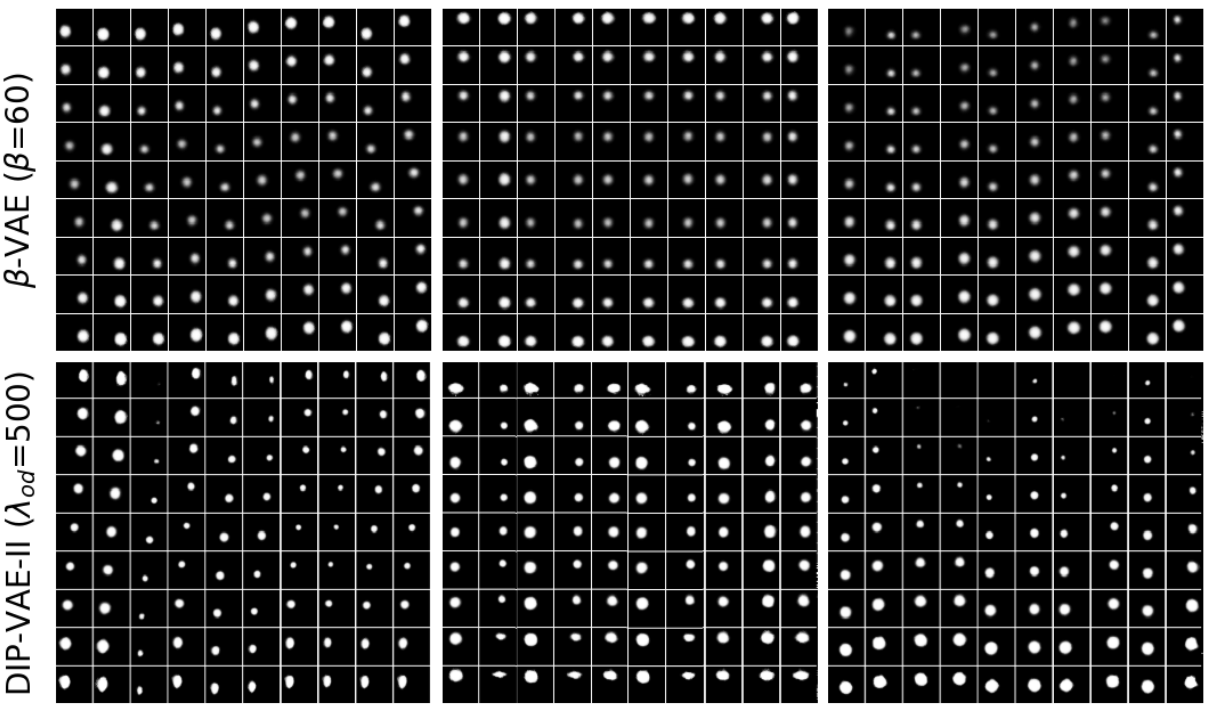
\includegraphics[width=\linewidth]{figs/dip-vae_1}
	\end{figure}

	\myfootnotewithlink{https://arxiv.org/abs/1711.00848}{Kumar A., Sattigeri P., Balakrishnan A. Variational Inference of Disentangled Latent Concepts from Unlabeled Observations, 2017}
\end{frame}
%=======
\begin{frame}{Challenging Disentanglement Assumptions}

\begin{block}{Theorem}
	Let $\bz \sim P$ with a density $p(\bz) = \prod^d_{i=1} p(z_i)$. Then, there exists an \textbf{infinite} family of bijective functions $f : \text{supp}(\bz) \rightarrow \text{supp}(\bz)$:
	\begin{itemize}
		\item $\frac{\partial f_i(\bz)}{\partial z_j} \neq 0$ for all $i$ and $j$ ($\bz$ and $f(\bz)$ are completely entangled);
		\item $P(\bz \leq \bu) = P(f(\bz) \leq \bu)$ for all $\bu \in \text{supp}(\bz)$.
	\end{itemize}  
\end{block}
Consider a generative model with disentangled representation $\bz$.
\begin{itemize}
	\item $\exists$ $\hat{\bz} = f(\bz)$ where $\hat{\bz}$ is completely entangled
	with respect to $\bz$.
	\item The disentanglement method cannot distinguish between the two equivalent generative models:
	\vspace{-0.3cm}
	\[
		p(\bx) = \int p(\bx | \bz) p(\bz) d\bz = \int p(\bx | \hat{\bz})p(\hat{\bz}) d \hat{\bz}.
	\]
	\vspace{-0.6cm}
\end{itemize}
Theorem claims that unsupervised disentanglement learning is impossible for arbitrary generative models with a factorized prior.

\myfootnotewithlink{https://arxiv.org/abs/1811.12359}{Locatello F. et al. Challenging Common Assumptions in the Unsupervised Learning of Disentangled Representations, 2018}
\end{frame}
%=======
\begin{frame}{Challenging Disentanglement Assumptions}
	\begin{figure}
		\centering
		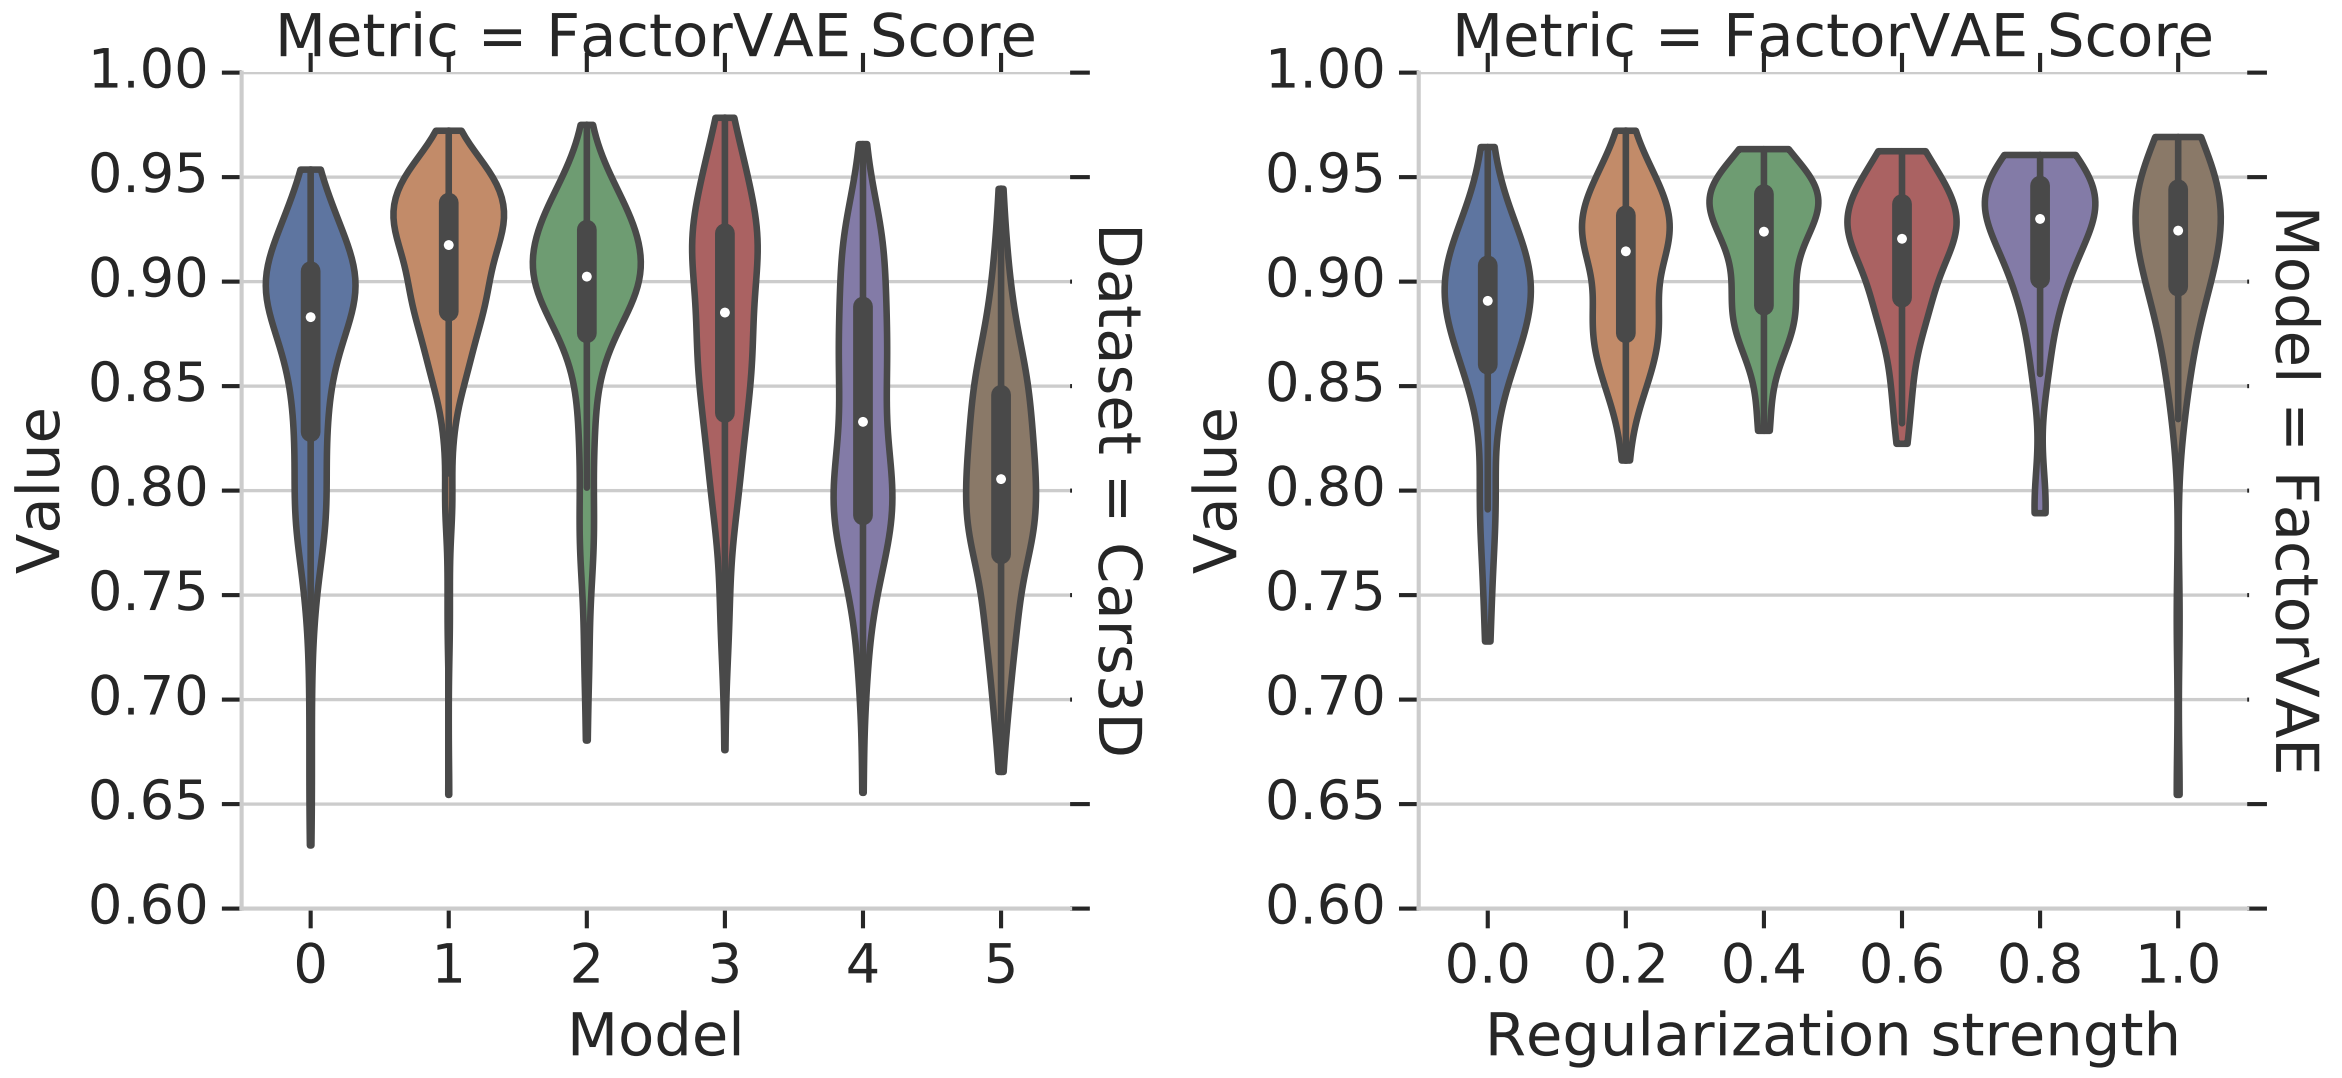
\includegraphics[width=0.85\linewidth]{figs/challenge_dis_2}
	\end{figure}
	\vspace{-0.3cm}
	\begin{figure}
		\centering
		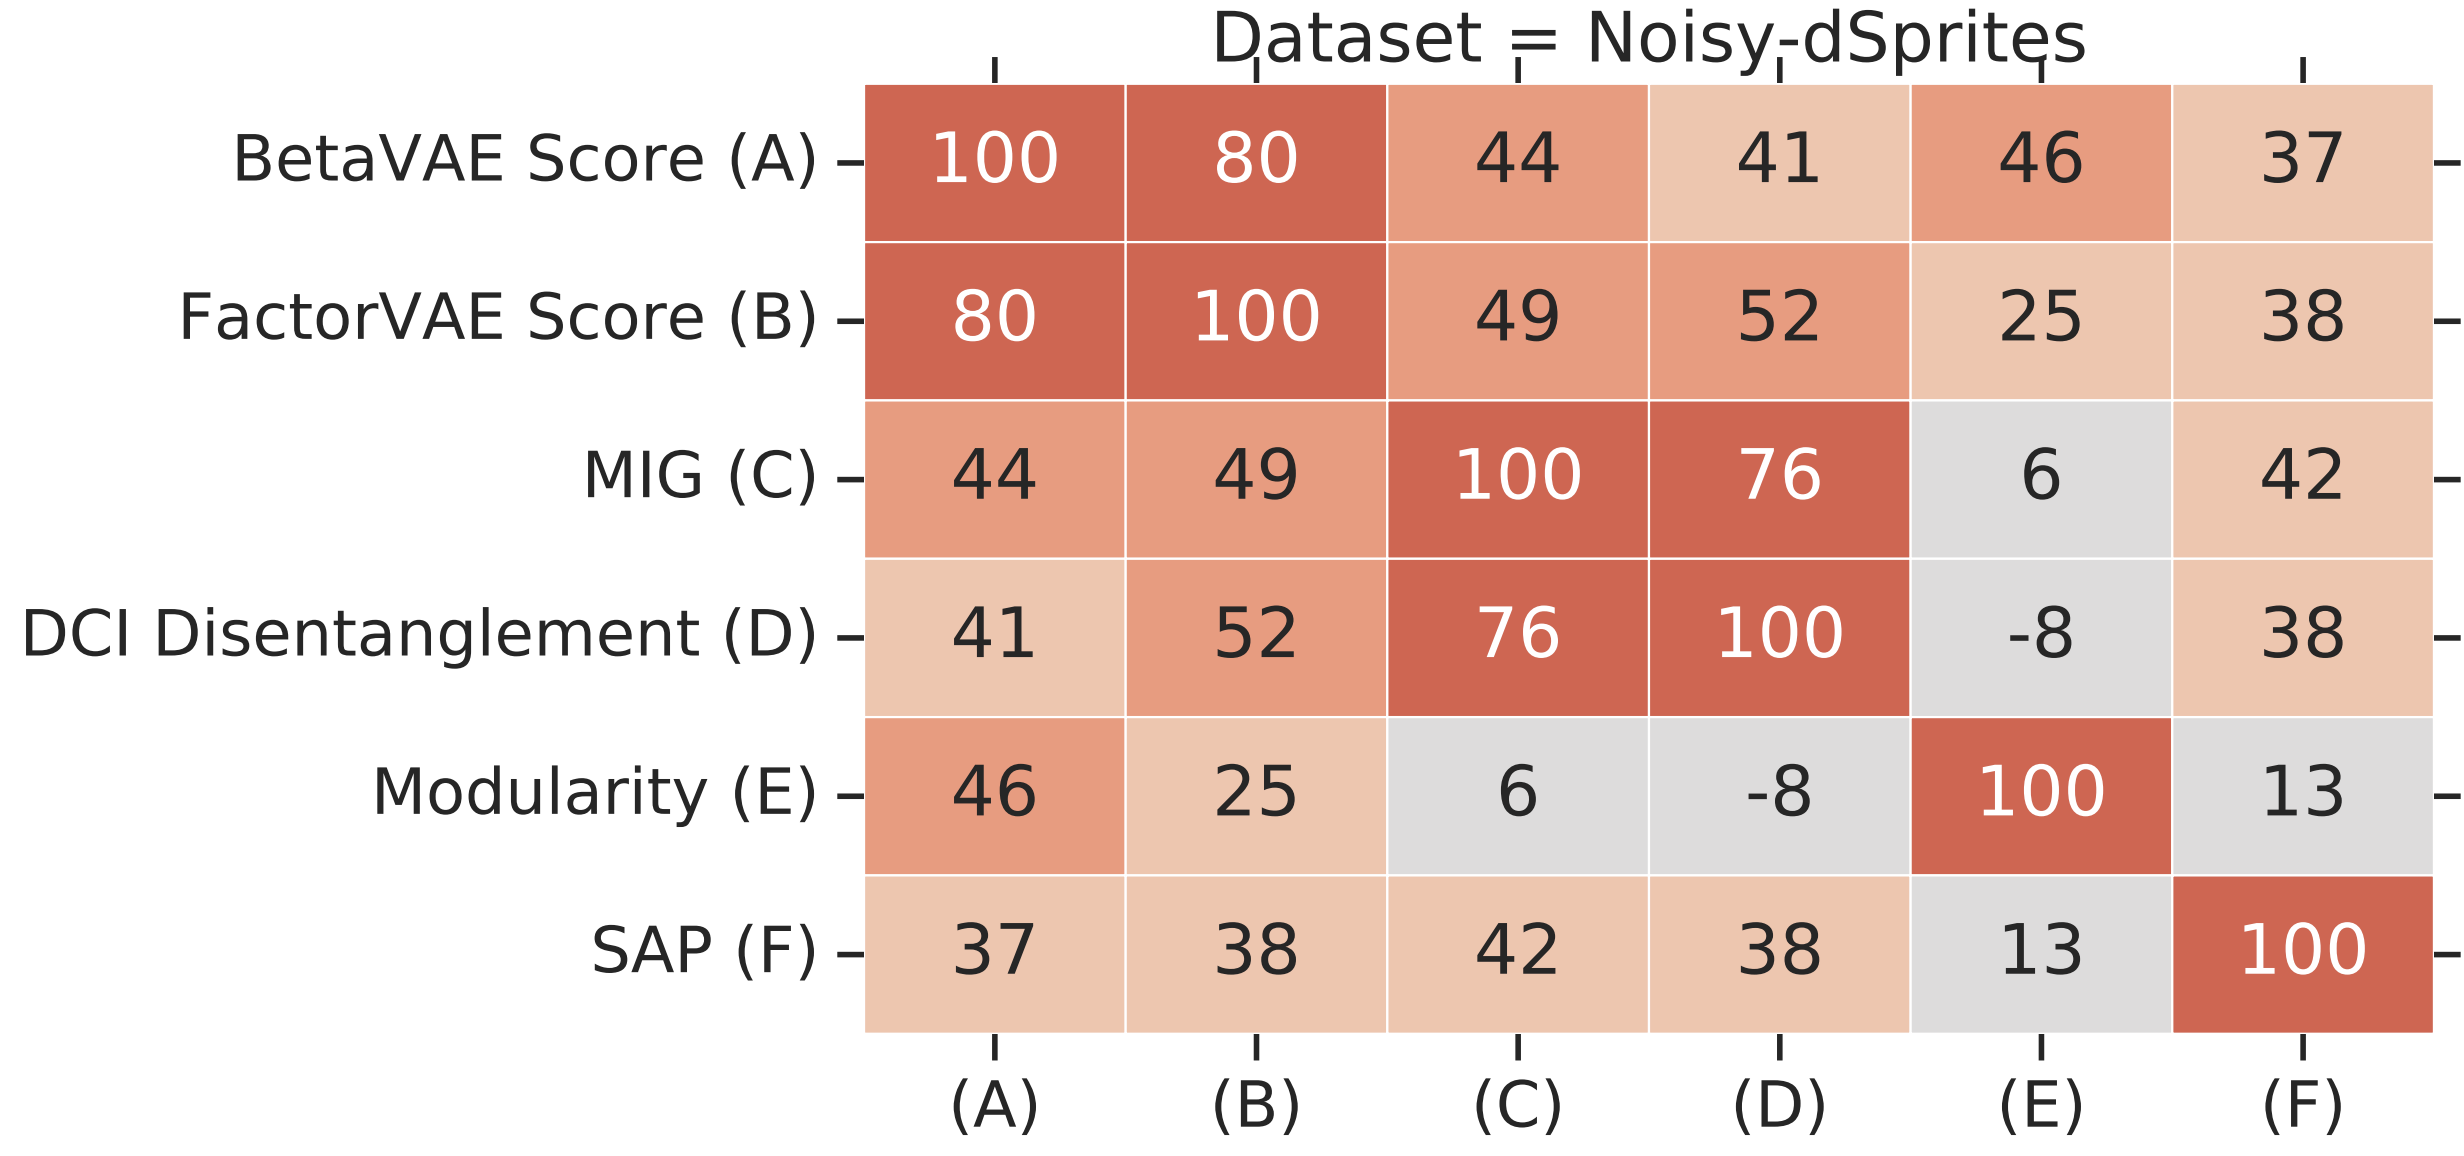
\includegraphics[width=0.65\linewidth]{figs/challenge_dis_3}
	\end{figure}

\myfootnotewithlink{https://arxiv.org/abs/1811.12359}{Locatello F. et al. Challenging Common Assumptions in the Unsupervised Learning of Disentangled Representations, 2018}
\end{frame}
%=======
\begin{frame}{Summary}
	\begin{itemize}
		\item Dequantization allows to fit discrete data using continuous model.
		\vfill
		\item Uniform dequantization is the simplest form of dequantization. Variational dequantization is a more natural type that was proposed in Flow++ model.
		\vfill
		\item Disentanglement learning tries to make latent components more informative.
		\vfill
		\item $\beta$-VAE makes the latent components more independent, but the reconstructions get poorer.
		\vfill
		\item DIP-VAE does not make the reconstructions worse using ELBO surgery theorem.
		\vfill
		\item Majority of disentanglement learning models use heuristic objective or regularizers to achieve the goal, but the task itself could not be solved without good inductive bias.
	\end{itemize}
\end{frame}
\end{document} 